\documentclass[xcolor=dvipsnames]{beamer}
\usetheme[navigation]{UMONS}
\usepackage[utf8]{inputenc}
\usepackage{graphicx}
\usepackage{wrapfig}
\usepackage{caption}
\usepackage{hyperref}
\usepackage{url}
\usepackage{color}
\usepackage{tikz}


\renewcommand{\arraystretch}{1.9}
\newcommand{\green}[1]{\textcolor{ForestGreen}{#1}}
\newcommand{\red}[1]{\textcolor{red}{#1}}

\title{Blockchain}
\author[G.Jérémy, D.Arman, L. Semih]{Gheysen Jérémy, Davidyan Arman, Locqueneux Semih}
\date{24 Avril 2018}
\institute[]{%
 Faculté des Sciences\\
  Université de Mons
  \\[2ex]
  
\includegraphics[height=4ex]{UMONS}\hspace{2em}%
  \raisebox{-1ex}{
\includegraphics[height=6ex]{UMONS_FS}}
}

\begin{document}

\maketitle

\section{Introduction}

\begin{frame}{Historique}

\end{frame}

\begin{frame}{Définition}
\vspace{-1cm}
	\begin{center}
		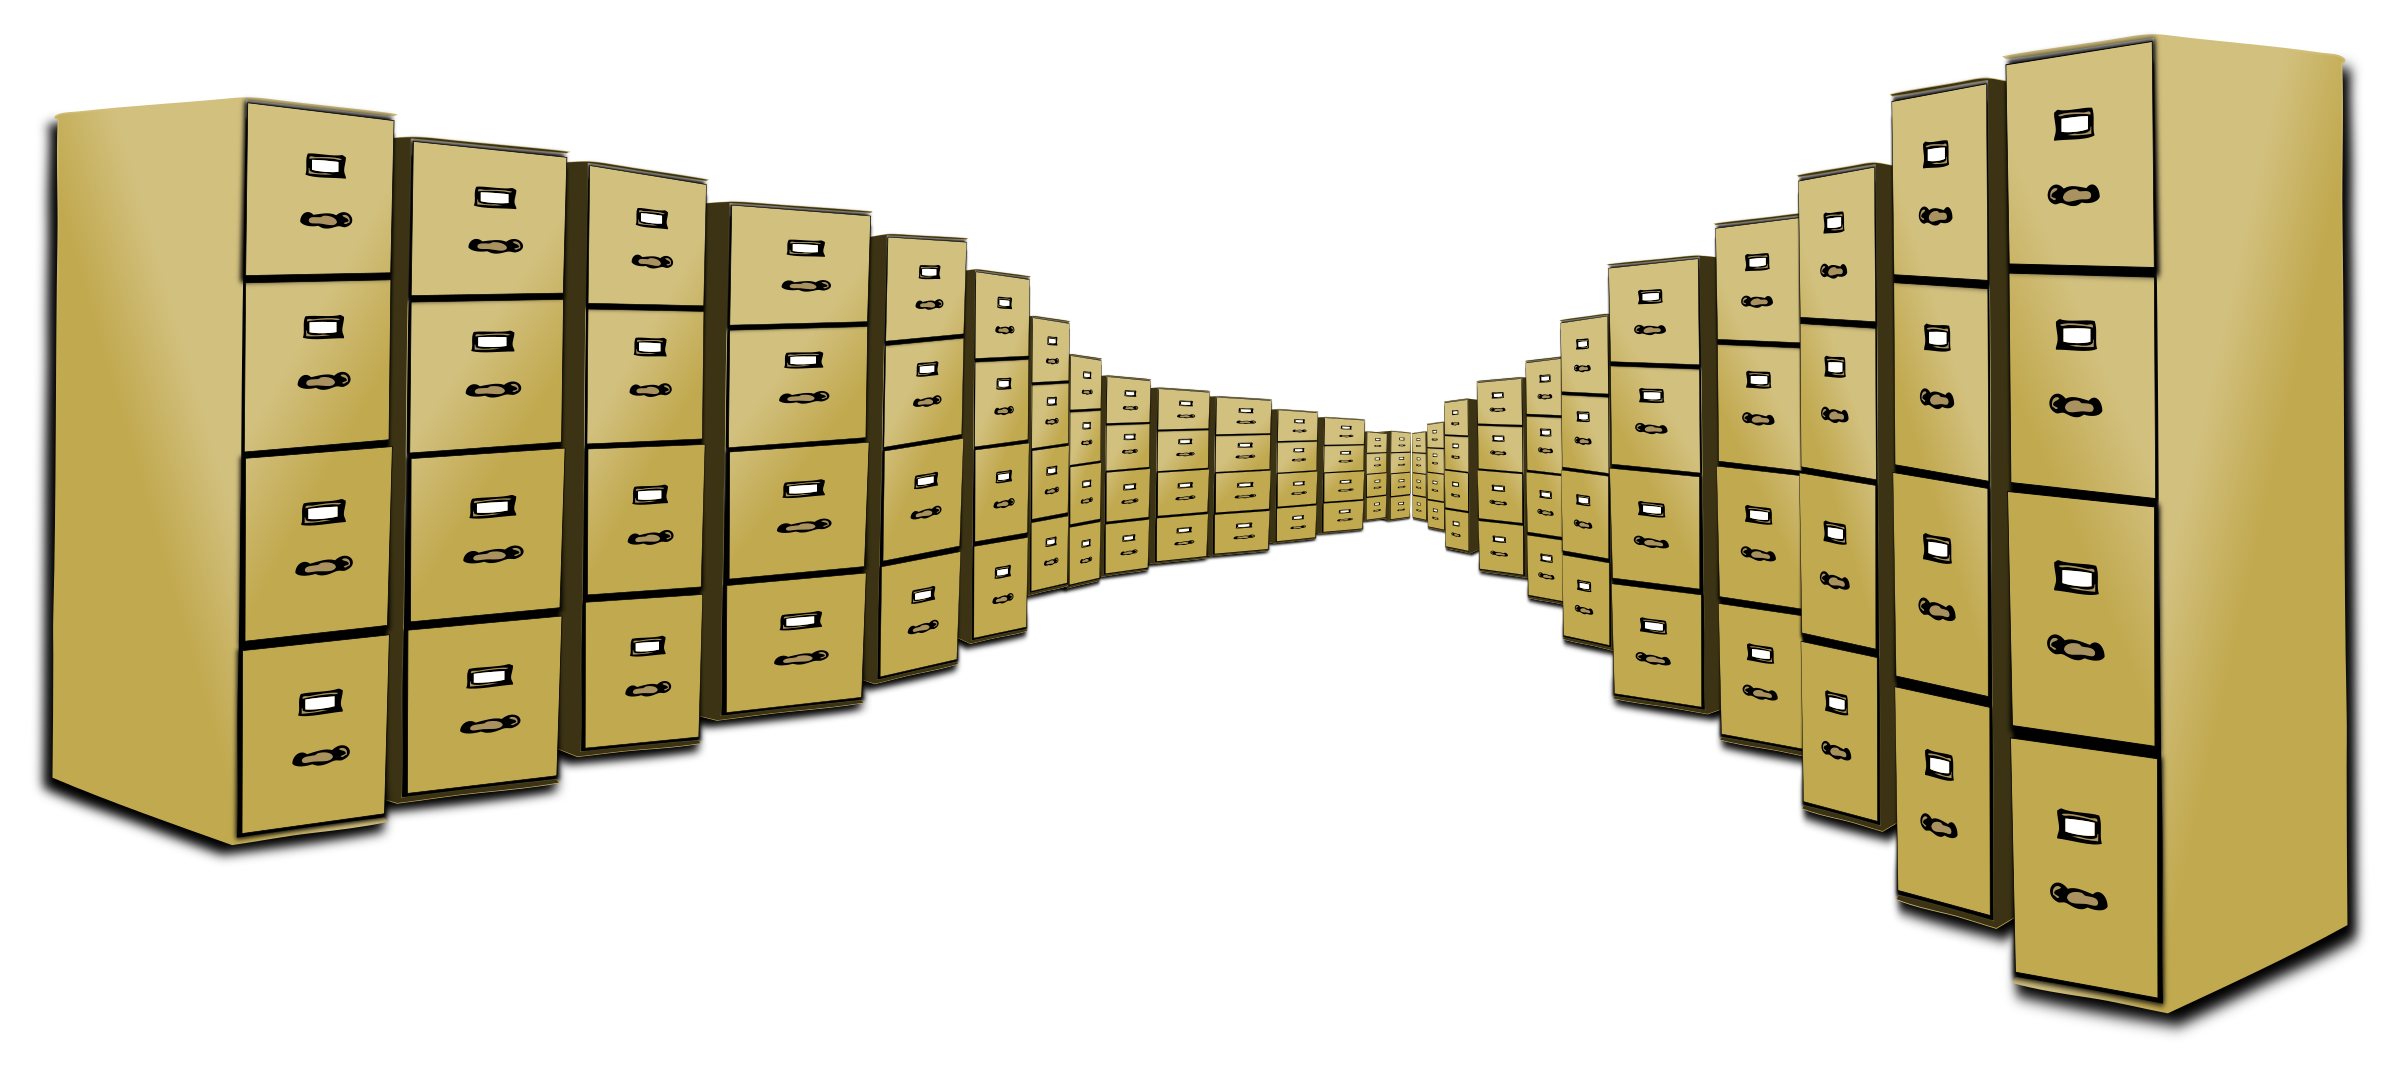
\includegraphics[scale=0.1]{storage.png} 
	\end{center}
	
	\begin{center}
	La blockchain est une technologie de \textbf{stockage} et de \textbf{transmission d’informations}, \textbf{transparente}, \textbf{sécurisée}, et fonctionnant \textbf{sans organe central de contrôle}.\footnote{\hspace{5pt}Définition de Blockchain France}
	\end{center}
	
	\begin{columns}
    	\begin{column}{0.48\textwidth}
    		\begin{center}
    			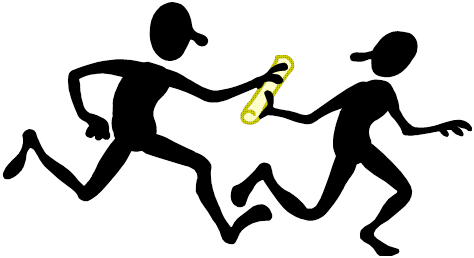
\includegraphics[scale=0.25]{relay.png} 
    		\end{center}
    	\end{column}
    	
    	\begin{column}{0.48\textwidth}
    		\begin{center}
				
\includegraphics[scale=0.25]{control.png} 
			\end{center}
    	\end{column}
	\end{columns}

% Liens  https://openclipart.org/detail/167738/filing-cabinet-overload
%		 http://worldartsme.com/relay-race-free-clipart.html#gal_post_57417_relay-race-free-clipart-1.jpg
%		 http://www.clipartpanda.com/clipart_images/security-bag-check-clip-art-58416511
\end{frame}

\begin{frame}{Objectifs}
	\vspace{-0.5cm}
	\begin{columns}
    	\begin{column}{0.48\textwidth}
    		\only<1-3>{
    		\begin{center}
    			\textbf{Durable\\}
    			\begin{figure}
    				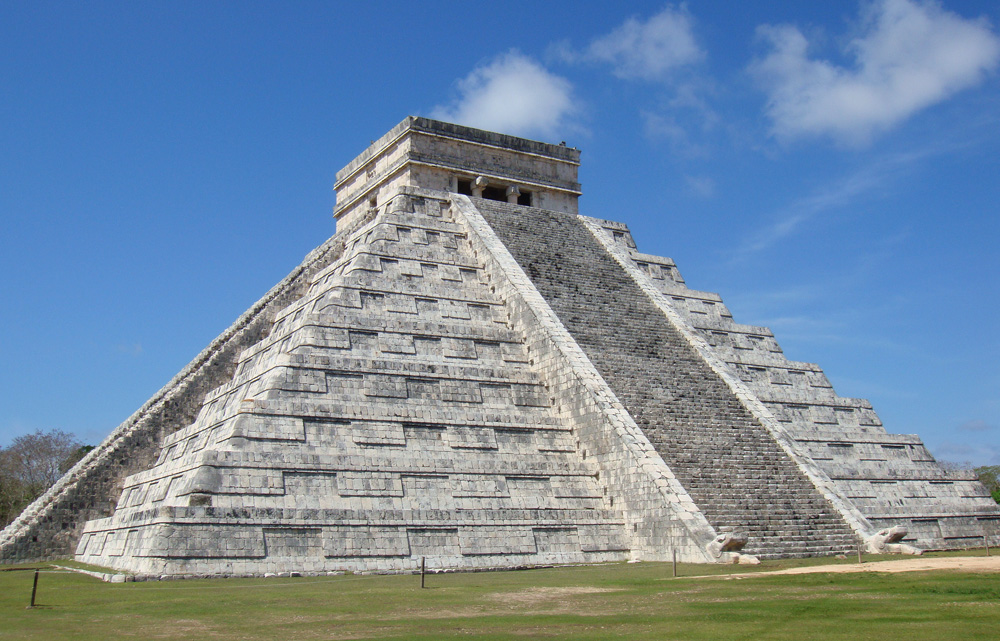
\includegraphics[scale=0.1]{perenity.jpg} 
    			\end{figure}
    		\end{center}}
    	\end{column}
    	
    	\begin{column}{0.48\textwidth}
			\only<2-3>{    		
    		\begin{center}
    			\textbf{Infalsifiable\\}
    			\begin{figure}
					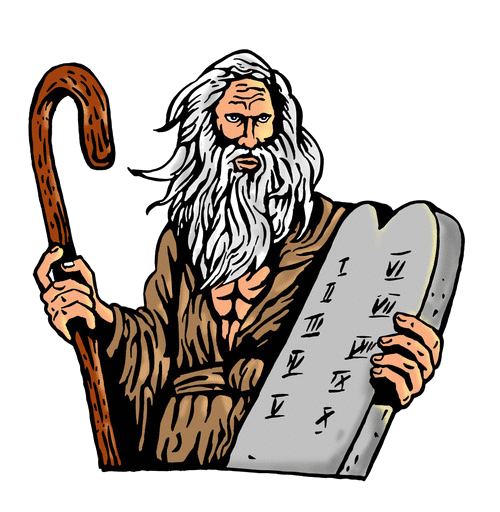
\includegraphics[scale=0.15]{commands.png} 
				\end{figure}
			\end{center}}
    	\end{column}
	\end{columns}
    		\only<3-3>{
    		\begin{center}
    			\textbf{Distribué\\}
    			\begin{figure}
    				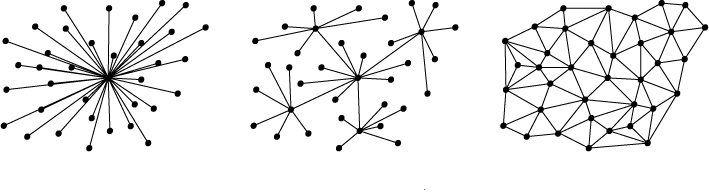
\includegraphics[scale=0.35]{central.png} 
    			\end{figure}
    		\end{center}}
% https://everestalexander.files.wordpress.com/2015/11/moses10commandmentstrans.gif
% http://zmeeed.info/aztec-architecture/popular-aztec-architecture-ancient-aztec-architecture-later-by-the-aztecs-th/
% http://blog.yintercept.com/2011/11/i-found-following-image-on-wikipedia.html
\end{frame}

\section{Smart Contract}

\begin{frame}{Smart Contract}
	
	
	\begin{center}
		Nick Szabo, \textit{Smart Contracts: Building Blocks for Digital Markets}, 1996
	\end{center}		
	
	\begin{figure}
		\centering
		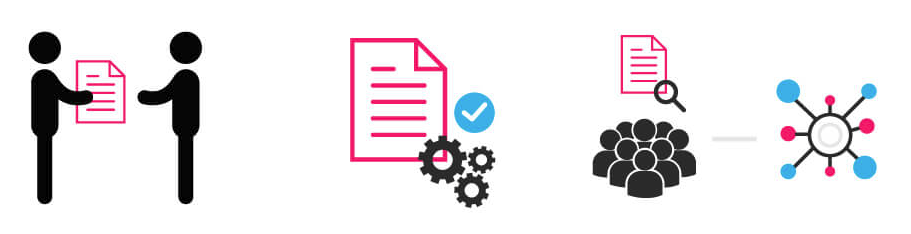
\includegraphics[scale=.25]{smart_contract}
		\caption{[Public domain]}
	\end{figure}
	
	
\end{frame}

\begin{frame}{Exemple d'Assurance}

	\begin{figure}
		\centering
		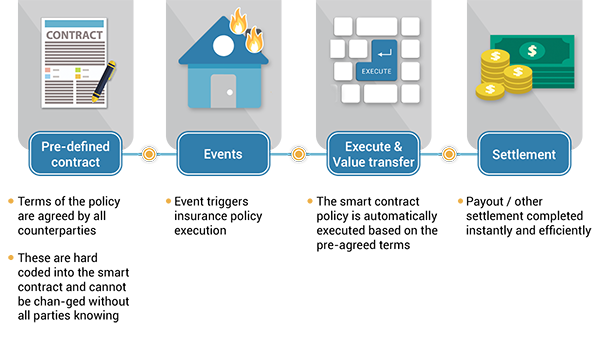
\includegraphics[scale=.5]{insurance_contract}
		\caption{By draglet GmbH [CC BY-SA 4.0 (https://creativecommons.org/licenses/by-sa/4.0)], from Wikimedia Commons}
	\end{figure}

\end{frame}

\begin{frame}{Exemple de code d'un contrat}

	\begin{figure}
		\centering
		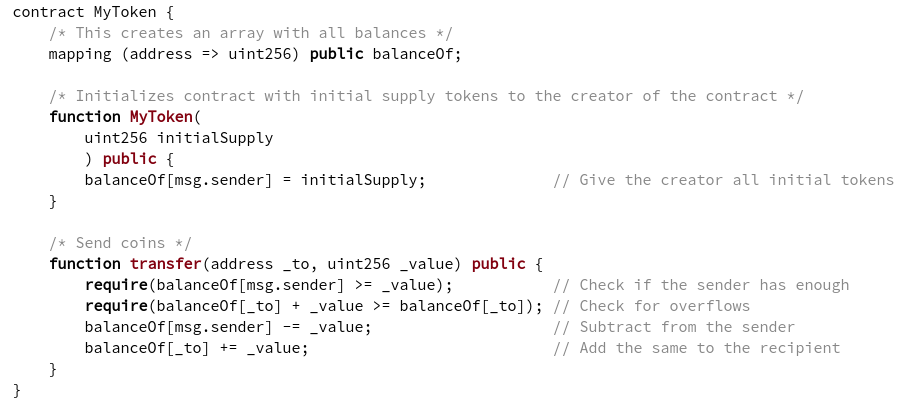
\includegraphics[scale=.35]{contract_example}
		\caption{exemple de smart contract sur Ethereum. Source: https://www.ethereum.org/token}
	\end{figure}

\end{frame}

\begin{frame}{Ethereum Tokens}

	\begin{center}
		\color{blue}
		Smart Contract de Ethereum permet de créer des blockchains sur base de leur blockchain
	\end{center}
	
	Exemple:
	\begin{figure}
	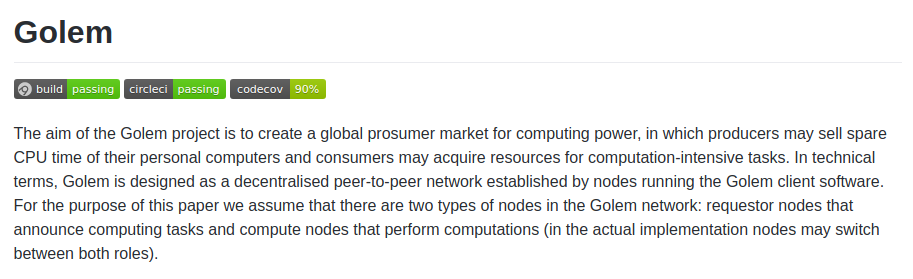
\includegraphics[scale=.35]{golem}
	\caption{source: page Github de Golem}
	\end{figure}

\end{frame}

\section{Conclusion}

\begin{frame}{Quelques Implémentations Intéressantes de Blockchain}

	\begin{itemize}
		\item L'Estonie a complètement digitalisé les données de leurs citoyens.
		\item Régulation du Commerce des poisson grâce à Hyperledger Sawtooth.
		\item Testing de smart cities à Dubai.
		\item Des votes éléctroniques à Moscou en 2014.
	\end{itemize}
	
\end{frame}

\end{document}